\documentclass[conference]{IEEEtran}

\usepackage{hyperref}
\usepackage{listings}
\usepackage{graphicx}
\graphicspath{{img/}}

\title{ARCAM-Net: A Software Defined Radio Mesh Network Testbed Implemented in GNU Radio with Batman-adv}
\date{2015-03-15}
\author{John McCormack, Bradley Trowbridge, Joseph Prine, R. Cody Maden, Ryan Integlia}

\author{
    \IEEEauthorblockN{John McCormack\IEEEauthorrefmark{1}, Bradley Trowbridge\IEEEauthorrefmark{2}, Joseph Prine\IEEEauthorrefmark{1}, R. Cody Maden\IEEEauthorrefmark{1}, Ryan Integlia\IEEEauthorrefmark{1}\IEEEauthorrefmark{2}}
    \IEEEauthorblockA{\IEEEauthorrefmark{1}College of Engineering, \IEEEauthorrefmark{2} College of Information and Technology}
    \IEEEauthorblockA{Florida Polytechnic Univeristy \\ Lakeland, FL, U.S.A.}
    \IEEEauthorblockA{\{johnmccormack2307, jprine2716, bradleytrowbridge06, randallmaden1497, rinteglia\}@flpoly.org}
}

\begin{document}
\maketitle


\begin{abstract}
	Cognitive Radio Networks (CRNs) seek to use systems of Software Defined Radios (SDRs) to establish
networks with flexible and intelligent physical and link layers. GNU Radio is an open source software
tool set for working with SDRs and CRNs.  Mesh networks are designed to allow for flexible and 
distributed network architectures to be self forming and to function without
the need for centralized infrastructure. Batman-adv is a popular open source layer 2 mesh network
protocol. Our work seeks to create a CRN by combinging GNU Radio with Batman-adv to create a fully open
source cognitivie radio mesh network. The platform can work with USRP SDR devices to quickly
prototype and experiment with cogntivie radio frameworks. Due to the flexibilty of Batman-adv
and GNU Radio, programs acting above Layer 2 can utilize this network without any changes.  


\end{abstract}
\begin{IEEEkeywords}
Software Defined Radio, ad-hoc network, mesh network, Software Defined Radio Network, SDR, SDRN, Batman-adv, USRP, Open-Mesh, A.L.F.R.E.D.,
GNU Radio
\end{IEEEkeywords}

\section{Introduction}

Software defined radios (SDRs) have been around for many years. However, as the cost of SDRs
continues to drop, the technology becomes much more accessible. Additionally, open source
tools such as GNU Radio make developing for SDRs much easier. GNU Radio provides a feature rich
ecosystem that provides a wealth of signal processing blocks. Though hardware is not a direct
component in GNU Radio, numerous other developers and projects have integrated hardware functionality
into the system either natively or through additional out-of-tree modules.

GNU Radio Companion allows for GUI development of PHY and MAC layer protocols within the
GNU Radio environment.The project itself is implemented in a combination of Python and C++ modules. 
Ettus research, a division of National Instruments, created the Universal Software Radio Peripheral 
(USRP) which is the SDR we chose for the project and a popular choice among many projects.
Ettus also released the Universal Hardware Drivers (UHD) which allow for the use of the USRP with GNU Radio.   

Cognitive Radio Networks (CRNs) are networks made up of SDRs that are capable of making 
intelligent decisions on their own and adjusting parameters such as signal strength. 
Many Cognitive Radio scenarios are designed around the idea of ad-hoc or mesh
networks. In these networks, all of the associated radio components are able to talk to each
other either directly or by "hopping" from one node to another until they reach their destination. 
The Better Approach to Mobile Ad-hoc Networks (BATMAN) project created the Batman-adv protocol. 
This layer 2 protocol has a fairly large community and is integrated into the Linux Kernel. 

Our goal with this project was to create a low cost, open source platform, that could serve as a
basis for future projects in Cognitive Radio Network research. Our hope is that by combining the GNU
Radio and Batman-adv projects, more collaborative research can be done with a standarized toolset. 
Our platform will also allow for students who are looking to create application layer products that 
leverage cognitive radio meshes to get started without having to worry about all the intracasies of
these networks. 

\section{Related Work}

\subsection{Software Defined Radio Testbeds}

There are several well known Software Defined Radio testbeds in use at different Universities. One major platform is the WARP platform from Rice University. This platform is made up of many custom components including the radio hardware itself \cite{7071706}. This makes the platform very expensive and limits its adaptability for use in other research groups. 

Another platform is the Hydra platform developed at UT Austin. This platform uses GNU Radio to define PHY Layer parameters and the Click Modular Router to implement Layer 2 protocols \cite{4212821}. The Hydra platform also uses USRP radios as the hardware frontend. However, Click is an older software which, according to their website, has not had an updated release since 2011 \cite{citationNeeded}. GNU Radio has since added the Polymorphic Tree (PMT) and Message types to allow for more Layer 2 development to be done right inside GNU Radio \cite{citationneeded}. 

The ADROIT project was another platform developed in conjunction with DARPA. This project relied heavily on Click and GNU Radio for much of its functionality. \cite{4286321}  Similarly, the University of California, Irvine and Boeing Corporation developed a testbed based off of USRP Radios and GNU Radio, but they implement custom MAC layers \cite{4753441}. 

The platform that most closely resembles ours is presented in \cite{0002}. However, this platform uses OLSR which has been shown to perform poorly when compared to Batman-adv. OLSR is also not truly decentralized as only certain nodes relay network information \cite{5375690}. 

\subsection{GNU Radio and Mesh Networks}

There has been work done in the past on establishing Mesh Networks using GNU Radio, however most of the research has had a different focus than ours. In \cite{4509617} and \cite{5062250} the authors use GNU Radio as a way to verify the succesful use of algorithms for mesh networking. However, they do not use SDRs,instead choosing to use GNU Radio for simulation. 

The researchers in \cite{7141228} created a simple multihop test bed using three USRP radios to relay data from one computer to another. A forth USRP acts as a primary user and attempts to block the signal. However, their work focuses on using reinforcement learning to allow for frequency hopping instead of focusing on a mesh routing protocol that can scale to more radios. 

Much of the existing work done using USRPs and GNU Radio for SDR Mesh Networks revolves around implementing different parts of the OSI protocol stack from the ground up. In some papers the authors focus on the physical or mac layer \cite{5508221}. There has also been work in developing new higher layer protocols for cognitive radio mesh networks such as work done to replace TCP with a more robust protocol \cite{6686523}. These systems will usually react to frequency changes but some also change their topology based on power use \cite{6983150}. All of this research is extremely important, does not create a complete platform to serve as the backbone for future work. 

\subsection{Mesh Network Testbeds}

The CONFINE platform uses Batman-adv as the routing protocol for their mesh network testbed. However,this testbed does not utilize GNU Radio or SDRS. \cite{0001} Batman-adv was also a key component of WiBed, a project to create a COTS mesh test bed using low cost wirelessrouters \cite{6686492} \cite{6962154}. Though they are not specific to SDR platforms, these still show the usefulness of Batman-adv as a component of a testbed. 
\section{Design}

The Design of the test bed can be broken down into the following parts:

\begin{figure}
	\centering
	\includegraphics[scale=0.25]{ProtocolStack}
	\caption{An overview of the components of the system, including the OSI Layers they interact with. \cite{0003} \cite{0007} \cite{0008} \cite{0015} \cite{0012} \cite{0011}}
	\label{fig:ProtocolStack}
\end{figure}

\begin{itemize}
	\item USRP Software Defined Radio
	\item GNU Radio Flowgraph
	\item Batman-adv
	\item Flask Web Server
	\item SocketIO Web Sockets
	\item A.L.F.R.E.D. 
\end{itemize}

This configuration is shown in Figure \ref{fig:ProtocolStack}

\subsection{USRP Software Defined Radio}

For our project, we utilized a combination of Ettus Research USRP B200 and USRP B210 SDRs. These radios are able to communicate from 70 MHz to 6 GHz and are well supported in GNU Radio using the open-source USRP Hardware Driver (UHD) provided by Ettus \cite{0007}. Their relatively low cost makes them ideal for building out larger testbeds. These serve as the radio transceiver for the current version of our platform. However, thanks to the UHD support in GNU Radio, any other USRP device will be compatible with the rest of the system, with little to no changes made to the development environment. 

\subsection{GNU Radio Flowgraph}

GNU Radio utilizes programs called ``Flowgraphs" to allow for graphical programming of SDR software. To implement the physical and link layers on the SDR, we utilize the Out of Tree (OOT) module gr-mac created by John Malsbury \cite{0015}. This flowgraph is a very simplistic, but effective, implementation of a Gaussian Minimum-Shift Keying (GMSK) or Orthogonal Freqency-Division Multiplexing (OFDM) transceiver with a mac layer protocol called ``simple mac". There are two main blocks in the flowgraph. The first sets up the GMSK or OFDM radio. This hierarchical block is built by running a separate flowgraph which contains the UHD blocks to interface into the USRP as well as the modulation and demodulation blocks for the waveform. One of the more important aspects of the two Radio blocks, is that they convert from streaming data to message data. 

Most features of GNU Radio work on streaming data where there is constant data transmission. However, packets are not sent continuously, therefore separate logic is needed to convert streams to messages. These messages are passed into and out of the GMSK and OFDM heirarchical blocks, so the remainder of the flowgraph deals with passing messages only. 

We use the GMSK block to convert from streaming data to message data and then connect this block to a tunnel (TUN) or network tap (TAP) interface block. TUN/TAP devices are virtual network kernel devices supported entirely in software. TUNs are used to simulate layer 3 devices and TAPs simulate layer 2 \cite{0017}. Either of these could be selected to suit the users purpose, but as batman-adv is a layer 2 protocol, we will use the TAP protocol. This flowgraph also implements an 802.3 Tracker to build out a radio to address map of the network. 

\subsection{Batman-adv}

Batman-adv was chosen based on its large community and documented success as a mesh routing protocol \cite{5375690}. It is already included as part of the Linux Kernel, and additional software can be downloaded from most distributions repositories \cite{0008}. Configuring batman-adv to work on the SDR involves running the program batctl and selecting the recently generated TAP interface created by GNU Radio. The Maximum Transmission Unit (MTU) of the TAP interface must also be changed to 1532 from 1500 in order to incorporate the additional header batman-adv uses when sending data. With just Batman-adv and GNU Radio, we are able to create a Software Defined Radio based mesh network. The remainder of the test bed was implemented to leverage features unique to GNU Radio and Batman-adv to create a method of sharing frequency and other data. 

\subsection{Flask Web Server and Socket.IO}

\begin{figure}
	\centering
	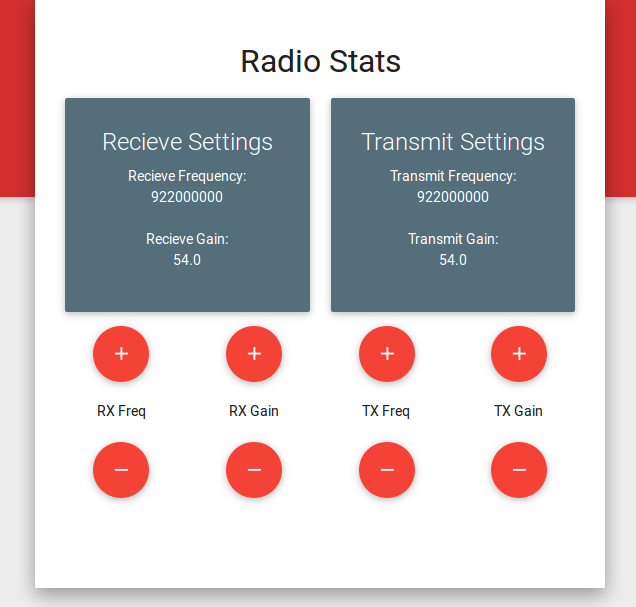
\includegraphics[scale=0.25]{WebInterFace}
	\caption{The web interface that lets the user initiate the network to hop to a new frequency.}
	\label{fig:WebInterface}
\end{figure}

Flask is a lightweight, open source, web framework for the Python programming language \cite{0011}. Flask was used to act as a broker between GNU Radio and any other user space applications or control systems we wished to implement. The Flask server runs the GNU Radio flowgraph in a background thread, while simultaneously configuring the TAP interface, setting up batman-adv, and starting A.L.F.R.E.D. as a background process. 

Socket.IO is a JavaScript library that enables real-time bidirectional event-based communication \cite{0012}.  SocketIO was chosen as a means of relaying data between the flask server and other components of the system due to its speed, flexibility, and ability to broadcast messages to any connected client. Socket.IO also integrates into Flask \cite{0013} and can be used in stock python with a client library \cite{0014}. In flask, we create wrappers to all the necessary GNU Radio parameters so that external tools can relay data to and from GNU Radio over web sockets.  

We also use flask to host a single webpage that displays various settings about the radio, and allows for the user to change parameters. The interface is shown in Figure \ref{fig:WebInterface} Since our platform does not yet include logic for automatic detection of primary user's, we simulate this by allowing a person to click a button to change to a new frequency. This frequency will then be sent to the Flask server using web sockets.  

\subsection{A.L.F.R.E.D.}

 The ``Almighty Lightweight Fact Remote Exchange Daemon," or A.L.F.R.E.D., is a system for distributing data to all nodes on a mesh network \cite{0015}. A.L.F.R.E.D. is very simple to use, but still powerful. Whenever a node writes data to a channel on A.L.F.R.E.D., that data is passed between each node so that all members of the network receive the data. Typical uses for A.L.F.R.E.D. include keeping track of sensor data or building a visual map of the network. 

 An additional feature of A.L.F.R.E.D. is its ability to pass a command to the command line whenever new data is added. When the transmission frequency of the USRP is changed on the Flask server, Flask sends this information along with a UTC timestamp to A.L.F.R.E.D. before changing frequencies. A small delay is created so that we can be sure the information was sent to the other nodes before the node changes its broadcast frequency.  

 When the other nodes receive the updated data table, A.L.F.R.E.D.'s callback function will run. This is a short program that parses the A.L.F.R.E.D. data table and looks for the most recent data it received. The callback function then sends the new frequency to Flask using Socket.IO which causes Flask to change the frequency in the GNU Radio flowgraph.   
\documentclass{IEEEtran}
\usepackage{lipsum}

\title{IEEE article}
\author{Theman Dlegend}

\begin{document}\maketitle
\lipsum[1]
See \cite{8} for more info 
\bibliographystyle{IEEEtran}
\bibliography{testing}
\end{document}

\section{Results}

\subsection{Network Benchmarks}

\begin{figure}
	\centering
	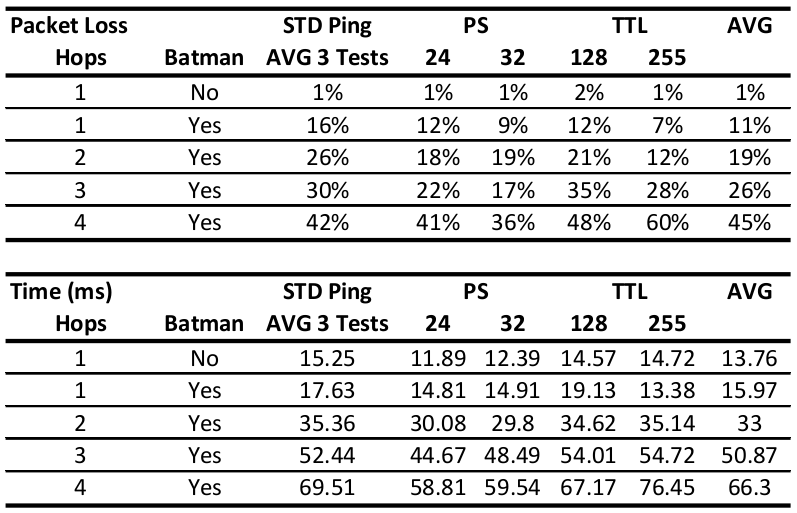
\includegraphics[scale=0.3]{902sheet}
	\caption{The data received from operating at 902/915 MHz.}
	\label{fig:902}
\end{figure}

\begin{figure}
	\centering
	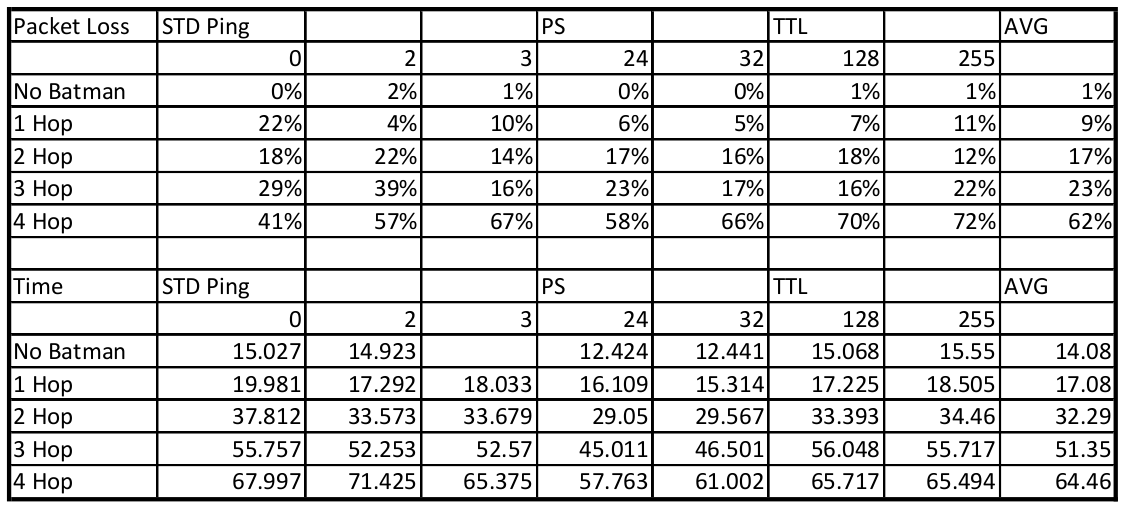
\includegraphics[scale=0.3]{2400}
	\caption{The data received from operating at 2.4/2.5 GHz.}
	\label{fig:2400}
\end{figure}

\begin{figure}
	\centering
	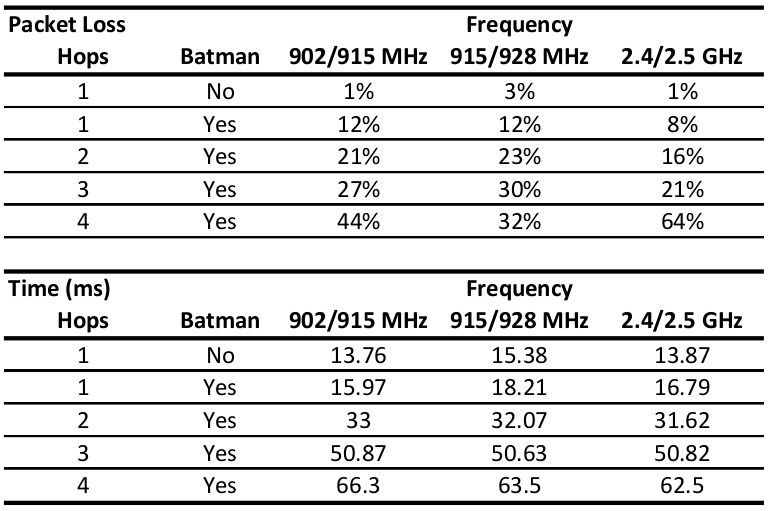
\includegraphics[scale=0.3]{alldata}
	\caption{The Averages from all three tests.}
	\label{fig:alldata}
\end{figure}

The results of the Network Benchmark tests are summarized in Figure \ref{fig:alldata}. In all cases, a single point to point communication, without the Batman-adv protocol running, resulted in a much lower packet loss. However, it is intersting to see that in the two sets of lower frequency raitings, the packet loss remained below 50\%. Also, the increase in time as hops were added has a roughly linear change. This is good as it means the overhead of adding more hops is not unmanageable. A full listing of tests run for the 902/915 MHz, and 2.4/2.5 GHz cases are provided in Figure \ref{fig:902} and Figure \ref{fig:2400} respectively. These tables show that running at the higher frequencies causes the SDRs to drop a lot more packets, especially when moving through the full four hops.  


\subsection{Route Changes}

\begin{figure*}
	\centering
	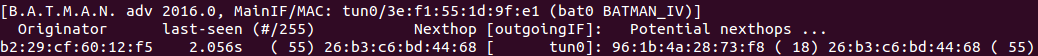
\includegraphics[scale=0.5]{2PotentialHops}
	\caption{The initial condition, where there are two possible routes the packet can take.}
	\label{fig:2Hops}
\end{figure*}

\begin{figure*}
	\centering
	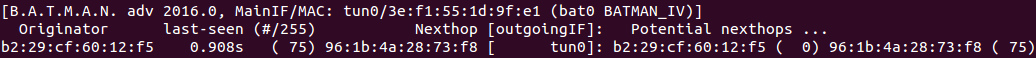
\includegraphics[scale=0.5]{hopchange}
	\caption{After the gain is reduced, the packets are now routing through a different node.}
	\label{fig:NewHop}
\end{figure*}

The route changing feature of Batman-adv worked very well with out test setup. As we decreased the gain of the intermediate node, the link quality reported by batctl also decreased. Eventually, Batman-adv switched and began using the other node. The initial setup can be seen in Figure \ref{fig:2Hops}. After the change, the routing table appeared as it does in Figure \ref{fig:NewHop}. This feature seems to work well even in the SDR system, and can likely be without much change.  

\subsection{Frequency Changes}

Using A.F.R.E.D. for frequency hopping showed mixed results. We were able to get the Nodes to change frequency in unison, but not reliably. A.F.R.E.D. itself is designed for a traditional Wi-Fi environment, and therefore does not have an expectation that the other nodes will become completely unreachable. We were finding that often times the nodes would switch well before A.F.R.E.D. had propagated the datatable to the other nodes. This would leave one node with an out of date table, meaning it would not make the frequency change. In the current iteration of the project, there was no way for these orphaned nodes to find the rest of the network again. Figure \ref{fig:freqshift} shows a situation in which four out of five nodes were able to make the jump, with one node remaining at the original frequency.




\section{Limitations and Future Work}

The results from our experiments show that the network is functioning as a multi hop SDRN. However, it is clear that more work needs to be done. In a deployed network, packet loss as high as is seen in this network would not be tolerated. Therefore, an important next step would be to examine how we can utilize machine learning and artificial intelligence to adjust parameters when these large packet losses are detected. It is likely that a change in frequency or amplitude could mitigate some of the packet loss. For example, if the loss is due to too many nodes operating on the same frequency, that set of nodes could change to a unique, unused frequency for the duration of the transmission and then switch back. This would be the beginning of the networks transition from a SDRN to a Cognitive Radio Network (CRN). 

Furthermore, it would be beneficial to either improve upon A.L.F.R.E.D. or reimplement certain features in a new way in order to handle the frequency changing. If we have each node wait for an acknolwedge from its immediate neighbors before changing frequency, that node could then change its operation knowing that the data will make it to the rest of the network. Batctl is already able to report the immediate next hop neighbors, so the program could use this information to only wait for acknolwedgements from neighbors instead of waiting for the entire network to be ready to change. A frequency change under these conditions would lead to a much more robust network change. In order for the current A.L.F.R.E.D. setup to function, a delay was needed to give the network time to respond. Therefore, an asynchronous acknowledge would likely speed up this transition as well. 


\section{Conclusions}

This work represents a first step in a longer term project to create a fully functioning SDRN. The work demonstrates the potential for using GNU Radio in conjunction with Batman-adv and other Open-Mesh solutions. As the work continues forward, we hope the testbed can serve as a collaboration point between GNU Radio and Open-Mesh. Both represent excellent next generation, open source, wireless solutions and could likely benefit from collaboration between the two projects. Our work can be used as an excellent starting point for anyone looking to get an SDRN up and running quickly to begin prototyping other sections of the tool chain. We plan on releasing the code as well as a handful of tools to help other researchers get started. We hope that this will serve as the first step in creating an equivalent Cognitive Radio Network platform and testbed. 
\section{Acknowledgments}

We would like to thank Dr. Harish Chintakunta, Dr. Anas Salah Eddin, and Dr. Jorge Vargas. We would also like to thank Jerome Sonnenberg and David Chester of Harris for their support. 


\bibliographystyle{IEEEtran}
\bibliography{Batman}
\end{document}
